\chapter{Конструкторская часть}
В этом разделе будут представлены схемы алгоритма Кнута-Морриса-Пратта и его модификации с использованием эвристики <<плохого>> символа


\section{Разработка алгоритмов}
На рисунках \ref{fig:kmp} и \ref{fig:lps} представлены схемы алгоритма Кнута-Морриса-Пратта и вспомогательной функции соответственно, а на рисунках \ref{fig:bm1} и \ref{fig:bm2} схема модифицированного алгоритма с использованием эвристики <<плохого>> символа.

\begin{figure}[h!]
	\centering
	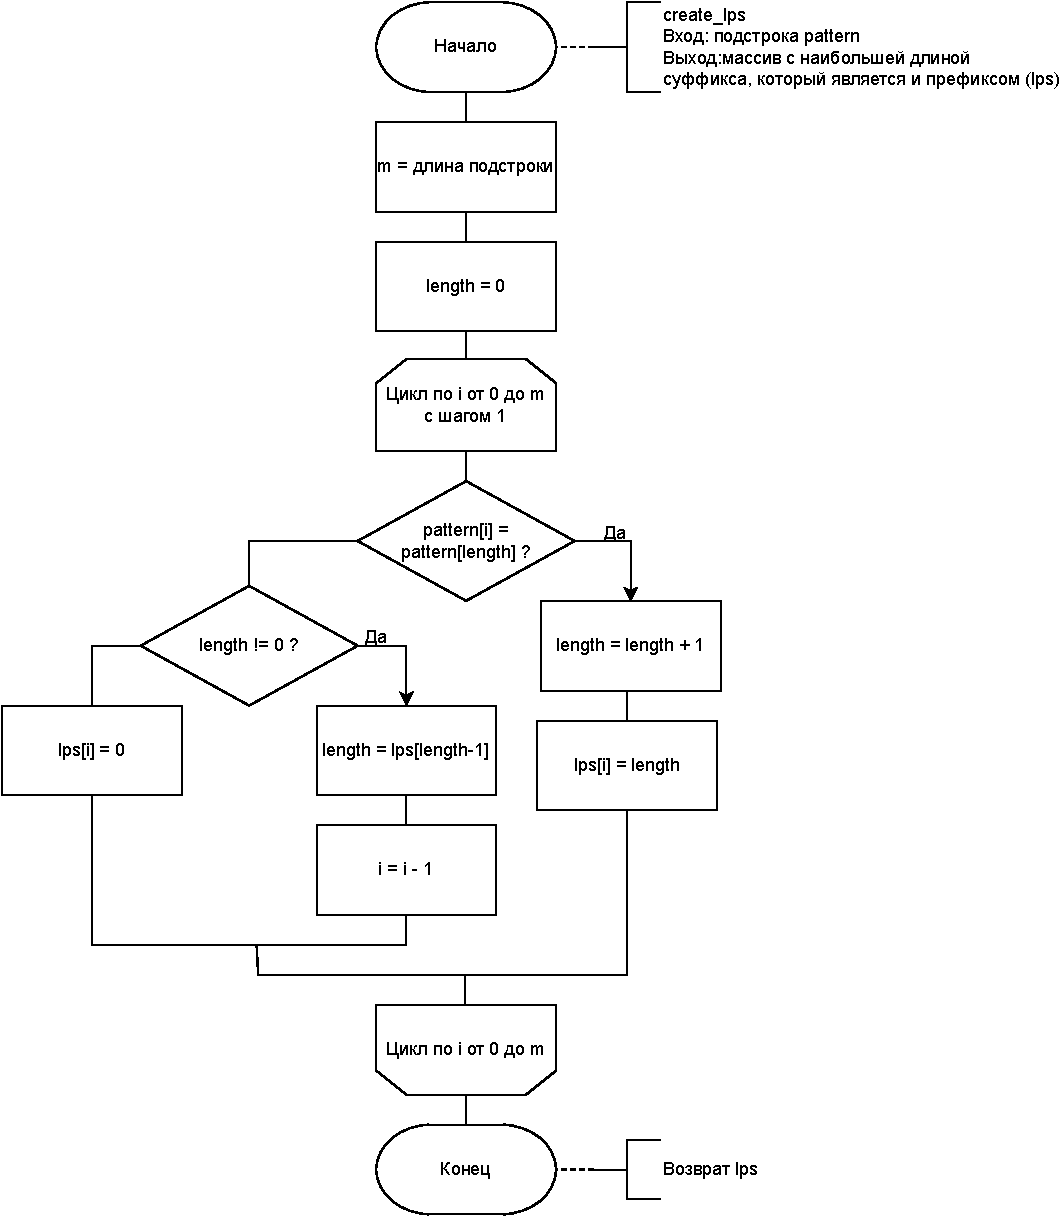
\includegraphics[width=0.78\linewidth]{img/lps}
	\caption{Схема алгоритма определения наибольшей длины суффикса подстроки}
	\label{fig:lps}
\end{figure}


\begin{figure}[h!]
	\centering
	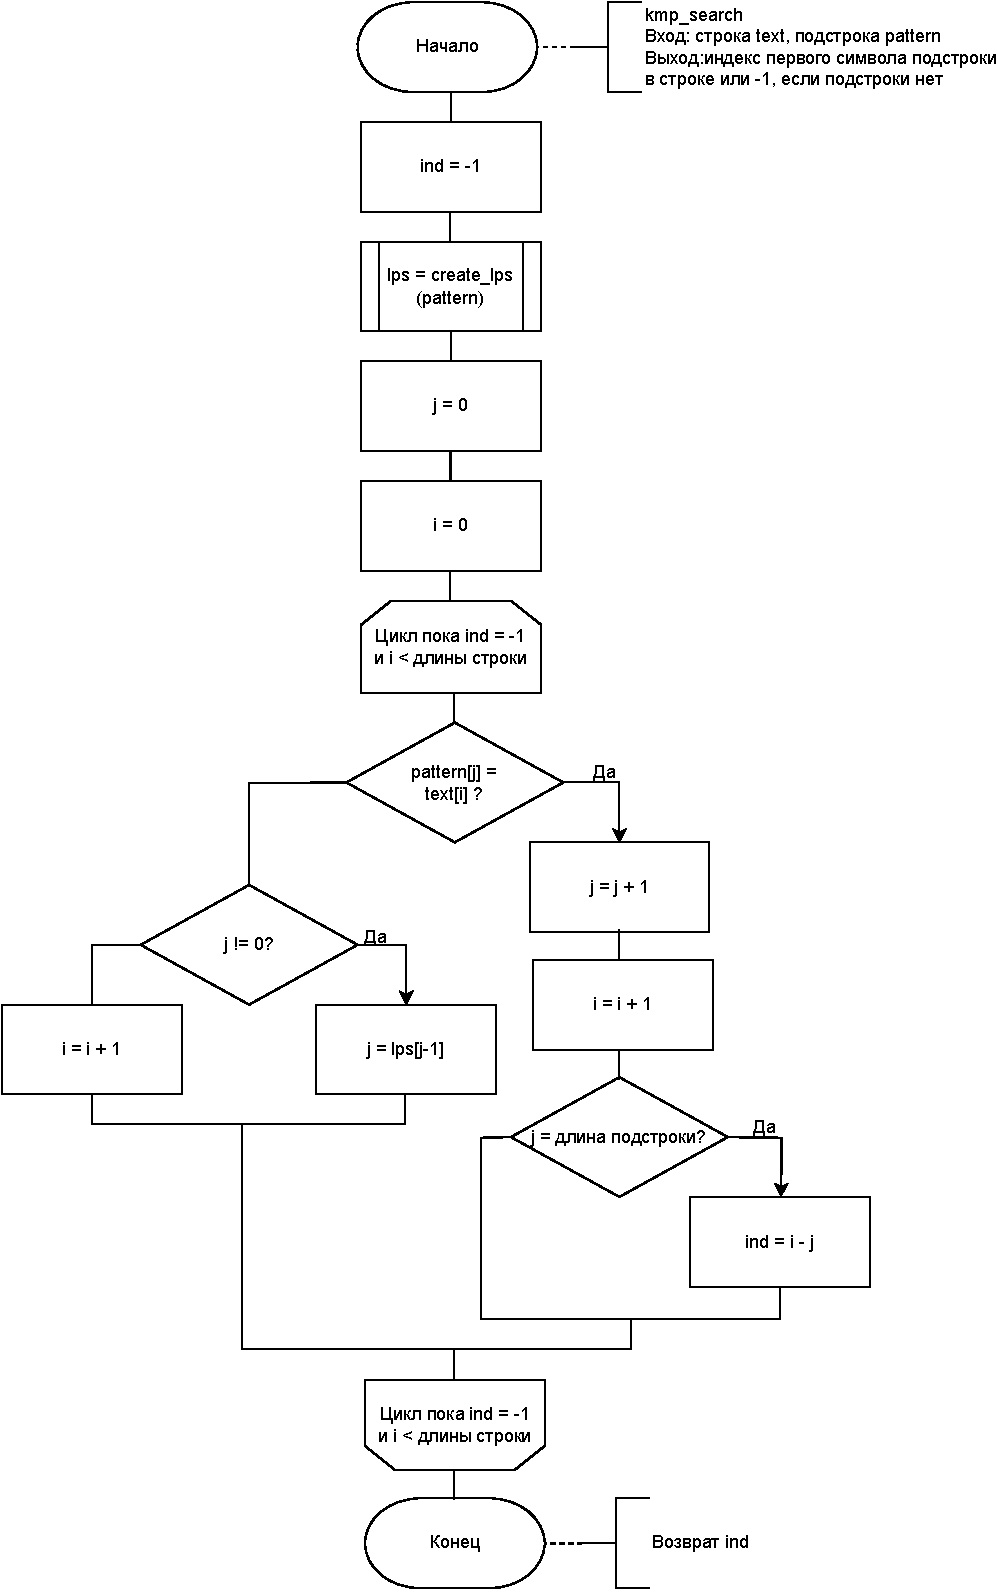
\includegraphics[width=0.9\linewidth]{img/kmp}
	\caption{Схема алгоритма Кнута-Морриса-Пратта}
	\label{fig:kmp}
\end{figure}

\begin{figure}[h!]
	\centering
	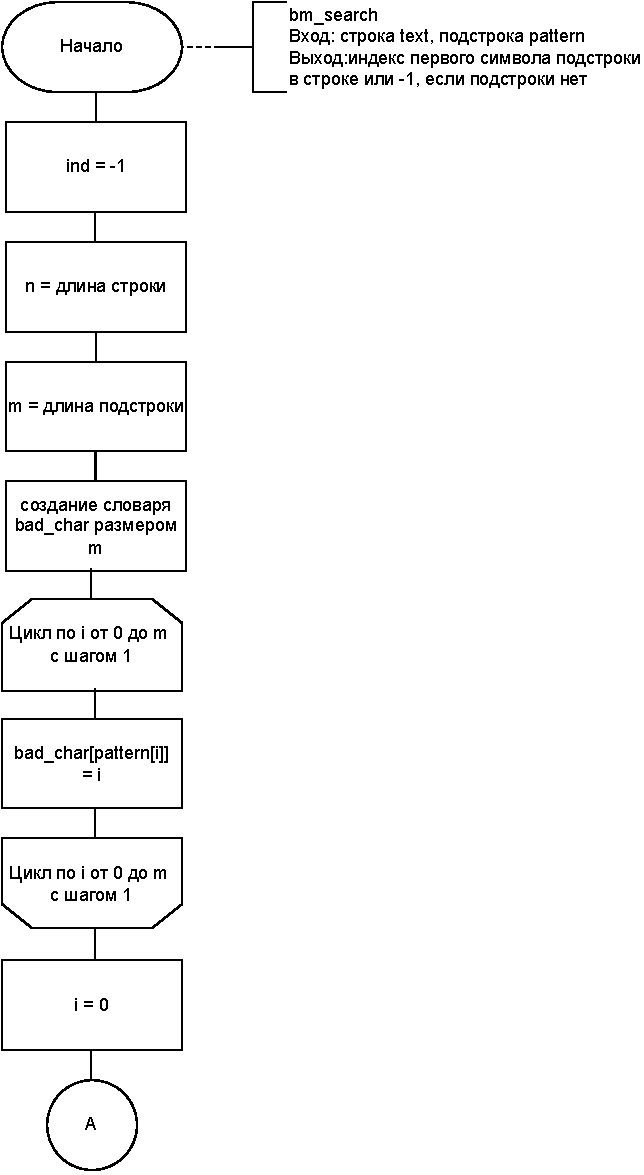
\includegraphics[width=0.8\linewidth]{img/bm1}
	\caption{Схема модифицированного алгоритма с использованием эвристики <<плохого>> символа(1 часть)}
	\label{fig:bm1}
\end{figure}

\begin{figure}[h!]
	\centering
	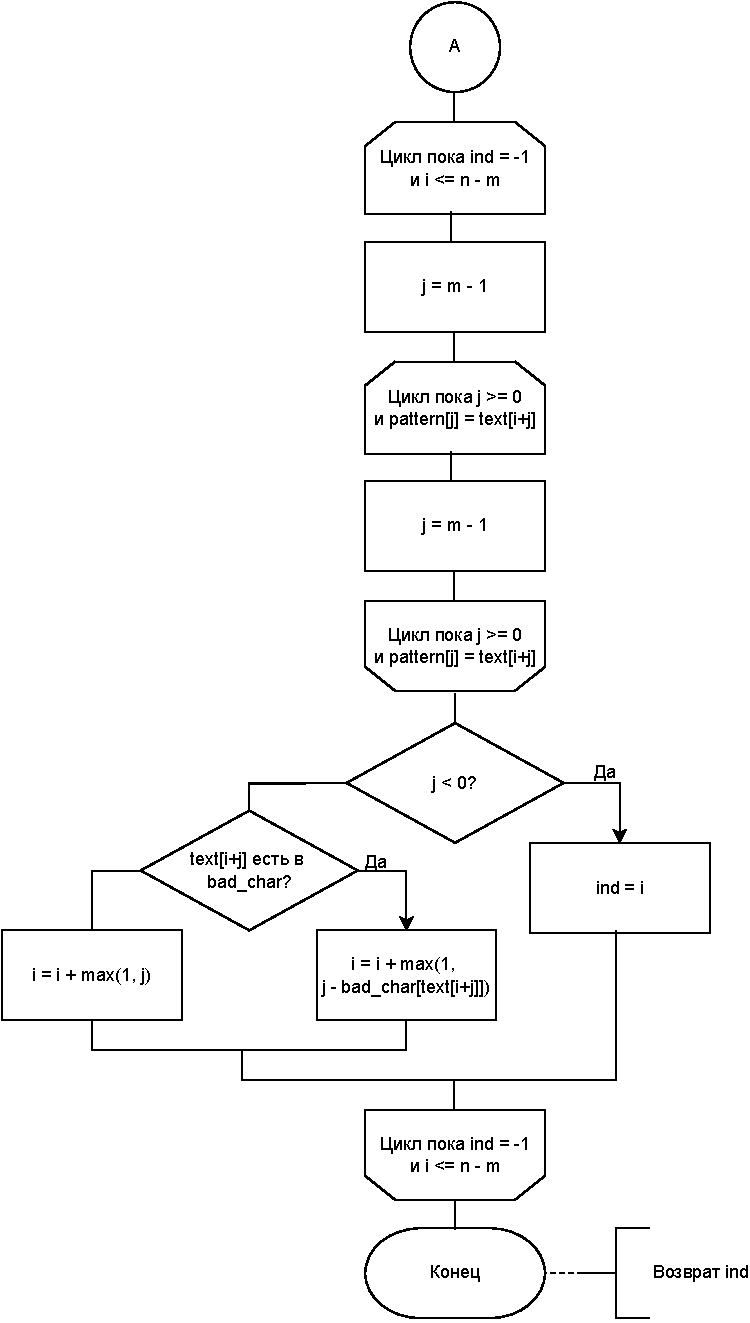
\includegraphics[width=0.8\linewidth]{img/bm2}
	\caption{Схема модифицированного алгоритма с использованием эвристики <<плохого>> символа(2 часть)}
	\label{fig:bm2}
\end{figure}
\clearpage


\section{Классы эквивалентности при тестировании}

Для тестирования выделены классы эквивалентности, представленные ниже.

\begin{enumerate}[label=\arabic*)]
	\item Неверно выбран пункт меню --- не число или число, меньшее 0 или большее 5.
	\item Неверно введена подстрока --- пустая строка.
	\item Неверно введена строка --- пустая строка.
	\item Подстроки нет в строке.
	\item Подстрока есть в строке.
\end{enumerate}


\section{Вывод}

В данном разделе были построены схемы алгоритмов, рассматриваемых в лабораторной рабо и были описаны классы эквивалентности для тестирования.
